
%%%%%%%%%%%%%%%%%%%%%%%%%%%%%%%%%%%%%%%%%%%%%%%%%%%%%%%%%%%%%%%%%%%%%%%
%                            Fifth Chapter                            %
%                   Evaluation and Experimentations                   %
%%%%%%%%%%%%%%%%%%%%%%%%%%%%%%%%%%%%%%%%%%%%%%%%%%%%%%%%%%%%%%%%%%%%%%%

\chapter{Evaluation and Experimentation}
\label{cha:evaluation_and_experimentation}

\graphicspath{{Chapter5-Evaluation/Figs/}}

%\section{List of contributions}
%\begin{itemize}
  %\item Understanding the environment through a point-cloud
    %Extraction of plane polygons from Kinect acquired point-clouds.
    %Segmentation pipeline:
    %\begin{itemize}
      %\item Acquisition
      %\item Filtering
      %\item Region growing segmentation
      %\item Planar Extraction
      %\item Planar projection and Hull convex generation
      %\item Re-orientation and transfer to the planner
    %\end{itemize}
  %\item Generation of sequences of postures on segmented environment
  %\item{Simulated scenarios planned on real-environment: HRP-2 climbing on table through stairs, HRP-2 climbing on table through slope}
  %\item{Machine Learning: Optimization of the solvers parameter for a class of problems}
    %\begin{itemize}
      %\item Developpement of a list of typical robotics optimization problem
      %\item Training of a genetic algorithm to find the "best" solver tuning to solve a family of problems
    %\end{itemize}
  %\item{Several scenarios, including Airbus}
%\end{itemize}

%\section{Application to contact planning on real environment}

%\subsection{Understanding the environment through a point-cloud}
%Segmentation pipeline:
%\begin{itemize}
  %\item Acquisition
  %\item Filtering
  %\item Region growing segmentation
  %\item Planar Extraction
  %\item Planar projection and Hull convex generation
  %\item Re-orientation and transfer to the planner
%\end{itemize}

%\subsection{Contact generation with convex surface inclusions}
%Usual methods for generating surface contact are based on point-to-point sampling, on rectangular inclusion, or other limiting methods. We proposed to extend that to the inclusion of convex surfaces.

%\subsection{Simulated scenarios planned on real-environment}
%We present 2 planned scenarios with the HRP-2 robot

In this chapter, we first present an approach to make use of posture generation in real-environment with data acquired directly from the robot.
And then, we study the performances of the method we presented to solve optimization problems on manifolds as well as the performances of our posture generator.

\section{Application of contact planning on real-environment}
\label{sec:application_of_contact_planning_on_real_environment}

Generating isolated postures is not sufficient to make a robot move or achieve tasks in ways similar to humans.
It needs to plan entire motions, with sequences of contact creations and releases, and trajectories in-between.
That's the role of the Multi Contact Planner (MCP).
The core of the planner consists in the multi-contact search and the posture generator.
The former incrementally builds a tree of contact sets and is presented in~\cite{escande:ras:2013}.
The children of a node are obtained by adding or removing exactly one contact to its set.
At each iteration of the search, the best leaf, according to a potential field, is expanded this way.
The tentative sets of contacts are tested by the posture generator: for a given set of contacts, it attempts to find a configuration of the robot that satisfies the constraints defined by the user (joint and torque limits, minimization of cost function, forces in friction cones, etc\ldots).
Upon success, the contact set is validated, and a new leaf is created.
The goal is written as a set of specific constraints.
A node is the final node if its associated posture generation problem augmented by these constraints remains feasible.
By backtracking from this final node to the initial root node, we obtain a sequence of nodes and thus a sequence of contact sets, that can be executed on the robot by a whole-body controller.
We make use of such a controller based on a quadratic programming (QP) formulation~\cite{bouyarmane:iros:2011}.

The potential field is derived from a crude path, made of a few key postures, that does not take contacts into account.
Such a path is either user-defined or can be the output of a first dedicated planner~\cite{bouyarmane:icra:2009}.

The MCP relies largely on the 3D geometric models of the environment and robotic agents.
In our previous work~\cite{escande:ras:2013,bouyarmane:ar:2012}, the geometric models are provided by the user.
The contact transition for the robot are planned off-line and later executed by the robot assuming exactness of the models and their relative positioning.
We aim at extending our MCP to deal directly with real data acquired by the robot.
Subsequently, we must deal with two kinds of situations:
\begin{enumerate}
  \item the models of the objects in the environment are known: in this case adapting the MCP consists mainly in dealing with recognition, model superposition and handling uncertainties.
  In brief, once model superposition is achieved, we can use the 3D model for MCP as in~\cite{escande:ras:2013,bouyarmane:ar:2012}, yet some adjustments are needed.
  \item the models of the hurdles and the environment are not known (e.g.\ disaster or outdoor environments, for example related to the Fukushima disaster that inspired the DARPA Robotic Challenge), MCP is to be achieved in an ego-centric way with models built from the robot's embedded sensors.
  This chapter deals with this case and we describe how the MCP is modified to achieve this goal.
  In a nutshell, we construct planar surfaces from the 3D point clouds data and feed them to the MCP.\@
\end{enumerate}

In robotics, the use of 3D-based vision for recognition and navigation in environment known or partially unknown has first been used on mobile robots, evolving in flat environment, for example by coupling it with a SLAM system~\cite{whitty:acra:2012}.
Another approach consists in extracting the surfaces from the point cloud, and then link them to the known environment or simply consider them as obstacles to be avoided~\cite{poppinga:iros:2008}.
Since working on raw point clouds is costly because of the high number of data points, this extraction has also been enhanced~\cite{biswas:icra:2012} in order to be run in real-time.
This approach has been recently experimented on a humanoid robot in~\cite{maier:humanoids:2012}, that combines two methods: the surface extraction from a point cloud, and the voxel-based 3D decomposition of the environment~\cite{nakhaei:humanoids:2008}.
Still, since the robot only navigates in a flat environment, and does not realize manipulation tasks, the surfaces extracted from the 3D point cloud are down projected to a 2D plan, on which are based the navigation and collision avoidance processes.

The use of humanoid robots allows to navigate in more complex environment, some work has been done to make a humanoid robot go down a ramp~\cite{lutz:iros:2012} or climb stairs~\cite{osswald:iros:2012}.
Yet, those methods use laser-based vision rather than point-cloud-based vision, so as to have a precise analysis of a known environment.

In this work, we aim at enabling a robot to analyze and plan a motion into a 3D environment.
Hence, we use the surface extraction of a point cloud to directly have a global picture of the environment and determine the convex planar surfaces that the robot can use at its advantage to progress using the MCP.\@
In our approach to make such an extension, we intentionally seek for technical solutions that minimize changes to be done on our existing MCP software.

\subsection{Building an understandable environment}
\label{sub:building_an_understandable_environment}

Our first concern is to build an environment that our multi-contact planner is able to ``understand'' and that can be extracted from a point cloud scene.
%The simplest kind of entity that our planner would be able to deal with is an oriented rectangular plan surface. Though, it is clear that the real world cannot be precisely described by such things, so we add another level of detail to our world description by using convex polygonal planar surfaces. Therefore, starting from an acquired point cloud, we try to extract a relevant set of such geometrical entities that will be our first description of the surroundings of the robot.

The simplest entity that our planner would be able to deal with and that could correctly describe the robot's environment is a set of convex polygonal planar surfaces.
Therefore, starting from an acquired point cloud, we to extract a relevant set of such geometrical entities that will be a first description of the surroundings of the robot.

In this section, we present the different steps we follow to create a set of relevant convex polygonal plane surfaces out of an acquired point cloud.
%\begin{itemize}
%\item Acquisition of the point cloud from a RGB and Depth sensor (see section~\ref{subsect:Acquisition})
%\item Filtering the point cloud(see section~\ref{subsect:Filtering})
%\item Plan extraction (see section~\ref{subsect:PlanExtract})
%\item Region growing segmentation(see section~\ref{subsect:region})
%\item Planar projection and hull convex generation (see section~\ref{subsect:PlanProjection})
%\item Re-orientation and transfer to the planner (see section~\ref{subsect:reorient})
%\end{itemize}

\begin{figure}
\centering
  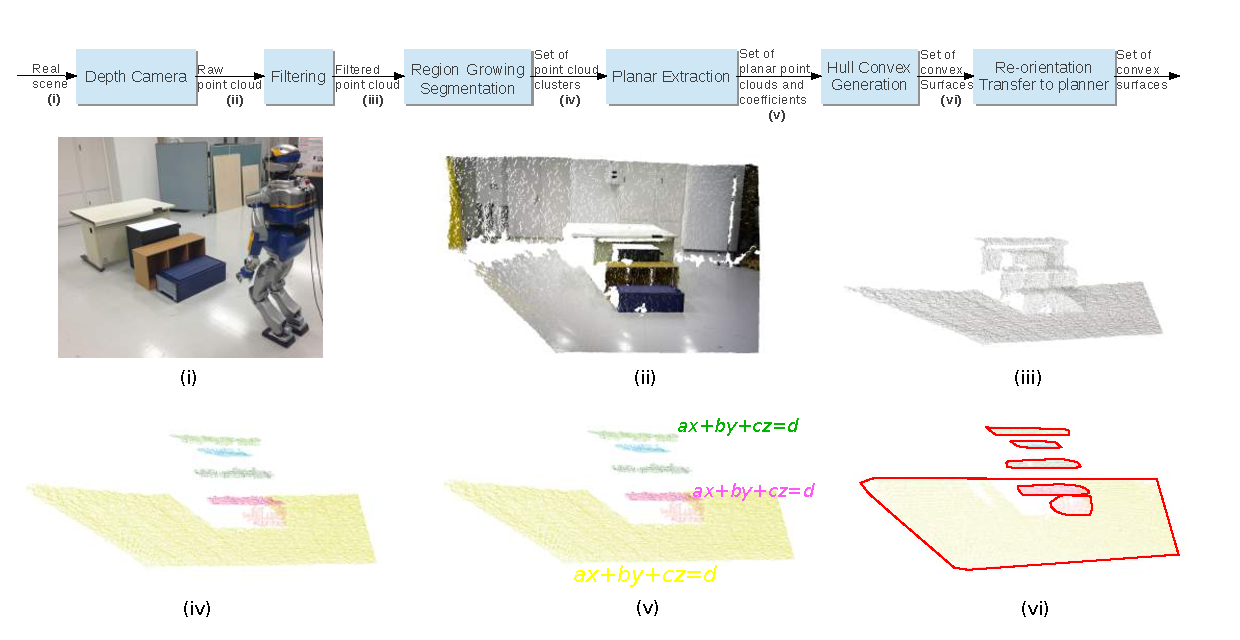
\includegraphics[width=\linewidth]{complete_pipeline.pdf}
  \caption{Top: flowchart describing the main elements of our algorithm and the type of data that is passed between them.\newline
  \hspace*{27pt} Bottom: the data throughout the process, illustrated in the case of our first experiment.}
\label{fig:full_pipeline}
\end{figure}

The Figure~\ref{fig:full_pipeline} illustrates the major steps of this point cloud treatment.
We use Willow Garage's Point Cloud Library\footnote{\url{http://pointclouds.org/}} (PCL)~\cite{rusu:icra:2011} extensively for processing the point cloud.

\paragraph{Acquisition of point cloud from a RGB and depth sensor}

The point cloud representing the scene is acquired by an Asus Xtion Pro camera.
The points are defined by their space coordinates and colors.
We do not use the color information for now except for display purpose.
It may however be useful for future developments in matching object models with sensor data and to perform color-based segmentation algorithms.

\paragraph{Filtering}

In order to reduce the computation time and improve the efficiency of our point cloud treatment algorithm we filter out the points that are too far and use a voxelized grid approach to downsample the remaining point cloud.
This consists in creating a 3D voxel grid over the point clout and replacing the points in each voxel by their centroid.
(We use this step to reduce the number of points to treat by a factor 5 to 6)

%, it is necessary to reduce the overall size of the data set. We first remove all points further than 5 meters from the camera: such points are not reliable enough and thus a potential source of error for the following steps.
%We know that the data extracted from the Asus Xtion live camera are reliable only for points that are less than 5 meters away from it. Therefore, we eliminate all the
%points that are further than that, since they would only be a source of error and wouldn't carry any valuable information.

%We then downsample the cloud, since it is excessively dense for our purpose. To do so, we use a voxelized grid approach (using the {\tt pcl::VoxelGrid} class): we create a 3D voxel grid over the input point cloud data. Each voxel represents a group of points that are close enough from each other to be represented by a single point that would be their centroid. The centroid is chosen instead of the center of the voxel because it represents the real environment more accurately. Another advantage of this method is that the filter can easily be parametrized by choosing the size of the voxels. Those two steps allow us to greatly reduce the number of points in the data set. Typically, in our experiments, this divides the number of points by a factor 5 to 6.

\paragraph{Region growing segmentation}

We divide a global point cloud scene into clusters of points that belong to the same flat area, by using a region growing algorithm~\cite{poppinga:iros:2008} that regroups the neighboring points that have similar normals into clusters.
%This method is based on the comparison of the angles between the points' normals.
%\note{\sout{This algorithm fits perfectly our needs, because it provides us with a list of sub-clouds (clusters), and each of those represents a flat area of the scene.}}
%It is used right before the planar extraction algorithm in order to obtain an accurate list of points and plane models they represent.

\paragraph{Planar extraction}

For each cluster, we use a plane segmentation to find the plan model that fits the highest number of points.
The outlying points can then be either filtered, or we can try to find another plan to fit them.

\paragraph{Planar projection and hull convex generation}

We extract the convex hull of the projection of each cluster on their respective fitting plan.
%The exact knowledge of all the data points contained in the plane model of a flat area is not necessary for our planning; we can reduce the point cloud to its convex hull without loss of information (except if the surface is concave, but this issue will be tackled in future works). In order to obtain the convex hull of each set of points, we first project every point of the set on its plane model ({\tt pcl::ProjectInliers} class) and then compute the 2D convex hull of the projected set of points ({\tt pcl::ConvexHull} class).
After this step, each plane surface of the scene is represented by a frame composed on the barycentre of the set of points and the convex hull of the surface.

\paragraph{Re-orientation and transfer to the planner}

After re-orienting each frame to get their expression with respect to the world frame, the list of \{frame + convex hull\} can be send to the planner as a list of contact surface candidates.
%Before sending the previously computed data to the planner, it is necessary to take into account the initial orientation of the camera. Indeed, if the camera was not aiming in a perfectly horizontal direction, then the entire point cloud would be misoriented. Therefore, it is necessary to re-orientate the surfaces before sending them to the planner. To do so, we simply apply a rotation matrix (that is computed from the initial camera orientation) to each of our data set's frame and origin to settle that problem. From there, the transfer of the surfaces to the planner can be done without any specific issue.

%Re-orientation is done as a last step for the sake of performance: obviously we need to re-orient only a few frames, compared to an early re-orientation of the point cloud that would require to apply a transformation on thousands of points.


\subsection{Constraints for surfaces extracted from point clouds}

Generating postures in which a contact between convex polygonal plane surfaces requires to ensure that the intersection area between the two surfaces is large enough to support the contact.
One could use the formulation presented in Section~\ref{sec:integration_on_non_inclusive_contacts_in_posture generation}.
Or more simply a constraint of convex polygon inclusion, which is sufficient for cases such as the ones we study here, where the support surfaces are wide enough for the robot to lean on.

%We adjusted slightly our planner and posture generator to handle contacts between convex polygonal plane surfaces.
%The main modification made in the posture generator deals with properly writing the constraints that enforce the inclusion of one surface into another one.
%In our previous implementation, contacts are searched between rectangular patches attached to the robot body or the environment.

Such constraint can be written by enforcing that all the points of polygon $S_i$ are located on the left side of all the segments of polygon $S_j$ (provided that the points of $S_j$ are ordered counter-clockwise around its normal).
For a couple of coplanar surfaces $S_i$, $S_j$ respectively represented by $n$ and $m$ points, this gives rise to a constraint of dimension $n \times m$:

\begin{algorithm}
\caption{Surface inclusion constraints}
\label{alg:surf_inclusion}
\begin{algorithmic}
\State{Let $S_i$ and $S_j$ be two coplanar plane surfaces}
\State{$S_i = {p_0, p_1, \ldots, p_n}$ and $S_j = {q_0, q_1, \ldots, q_m}$}
\State{$\vec{N}$ is $S_i$'s normal vector}
\For{$k = 0 \to n$}
\For{$l = 0 \to m$}
\State{Constraint $: \left[\overrightarrow{q_l p_k}\times\overrightarrow{q_l q_{l+1}}\right].\vec{N} \leq 0$}
\EndFor{}
\EndFor{}
\end{algorithmic}
\end{algorithm}

Once the surfaces are defined, it is possible to choose which ones are suitable for the robot to make contact with.
Although it is not a mandatory step, it allows to reduce the exploration during the planning phase by removing undesired or inappropriate pairs of robot/environment surfaces.
For the time being, this is determined by heuristics that are defined depending on the situation.
For example, if we want the robot to walk on various surfaces, only surfaces that have a normal vector closely aligned with the gravity field would be selected as potential candidates (so as to eliminate the walls and other surfaces on which the robot cannot walk).
Similarly, only surfaces located at a certain height can be considered for hand contact, etc.

For collision avoidance with the environment, we consider each surface generated by our point cloud treatment algorithm as a thin 3D body.
Basically, we extrude each surface by few centimetres in the direction opposite to its normal (provided that this normal is pointing toward the outside of the real body) and create a convex hull surface using {\tt QHull}~\cite{qhull:acm:1996}.
The collision avoidance is then computed by using the {\tt GJK} algorithm implemented in~\cite{benallegue:icra:2009}.
